\newpage
\textcolor{red}{Start with normal metal and look at its RKKY, then normal metal with SOC and RKKY, then SC with RKKY (follow Atousa on that one), finally SC with SOC and RKKY as perturbation.}
%%%%%%%%%%%%%%%%%%%%%%%%%%%%%%%%%%%%%%%%%%%%%%%%%%%%
\section{Normal Metal with RKKY interaction}
A normal metal can be described by a tight-binding model for fermions, which has the Hamiltonian
\begin{align}\nonumber
    H_{nm} = H_{kin} + H_{pot} = -t \, \sum_{\langle i,j \rangle, \sigma} c^{\dag}_{i,\sigma}c_{j,\sigma}  -\mu \, \sum_{i, \sigma} c^{\dag}_{i,\sigma}c_{i,\sigma}
\end{align}
with the annihilation [creation] operators $c^{[\dag]}_i$ for fermions with spin $\sigma$ at lattice site $i$, and the hopping amplitude $t$. 
Only nearest neighbor-hopping is included as indicated by $ \langle i,j \rangle$.
The lattice can be chosen freely and such that comparisons to possible experimental data become more easy.\newline
The potential energy of the system is proportional to the chemical potential $\mu$. \newline
The Hamiltonian can be diagonalized by transforming the fermion operators from real space to k-space via a Fourier-transformation of the form
\begin{equation} \label{eq:fouriertrafo_fermions}
    c_{i, \sigma} = \frac{1}{\sqrt{N}}\sum_{\vb{k}} e^{i\vb{k}\vb{r_i}}c_{k, \sigma}
\end{equation}
and its complex conjugate. 
For brevity, the vector $\vb{k} \in \mathbb{R}^3$ \textcolor{red}{Do I really have 3D here or is it only 2D?} going to be written as $k$ only.\newline
By defining the energy $\epsilon_k=-t\sum_{\langle i,j \rangle} \exp{(-i\vb{k}\delta_{ij})}$, the Hamiltonian can be expressed as
\begin{align}\label{eq:ham_normalmetal}
    H_{nm} = \sum_{k,\sigma, \sigma'} (\epsilon_k - \mu) c^{\dag}_{k,\sigma}c_{k,\sigma'}
\end{align}
The RKKY interaction as defined in Eq. \eqref{eq:RKKY_general} can also be Fourier transformed and then added to $H_{nm}$. 
That yields the expression
\begin{align}\nonumber
    H^{RKKY}_{nm} = \sum_{k,\sigma, \sigma'} (\epsilon_k - \mu) c^{\dag}_{k,\sigma}c_{k,\sigma'} + \sum_{k,k',\sigma, \sigma'} \sum_i \frac{J}{N}e^{i(k-k')r_i}(\vb{S}_i\cdot \Vec{\sigma}_{\sigma, \sigma'})c^{\dag}_{k,\sigma}c_{k',\sigma'}
\end{align}
where $r_i$ denotes the position of the impurity spin $\vb{S}_i$.
The added term containing the RKKY-interaction can be treated as a perturbation to the normal metal, which allows to use the SWT to obtain the effective interaction. \newline
After calculating the necessary commutators and taking the expectation value of the effective Hamiltonian, the spin structure can be identified as
\begin{align}
    \langle H^{RKKY}_{nm} \rangle = \langle H_{nm} \rangle - \sum_{i,j,k,k'} \left( \frac{J}{N}\right)^2 e^{i(k-k')(r_i-r_j)} \,2 \,\vb{S}_i \vb{S}_j \, \left(f(E_{k}) - f(E_{k'})\right)
\end{align}
where $f(E_{k,\sigma}) = \langle c^{\dag}_{k,\sigma}c_{k,\sigma} \rangle $ denotes the Fermi-Dirac distribution and $\langle H_{nm}\rangle$ is the expectation value for the unperturbed system.
This spin structure is of Heisenberg form and, consequently, the preferred orientation of the impurity spins is parallel without any preference regarding the axis, meaning that the system is isotropic in spin. \newline
The numerical solution presented in Fig. \ref{fig:spinstruct_nm_J2} displays exactly that behavior. 
The free energy of the system is the same for parallel orientation of the impurity spins, independent of distance and axis of alignment.
Nevertheless, the differences in free energy for different spin orientations decrease with increasing distance.
That can be explained by the fact, that the electrons can not travel entirely free within the metal and therefore loose information about the spin while moving from one to the other impurity spin. \newline
In Fig. \ref{fig:spinstruct_nm_J5}, parallel spin alignment is visibly favored for longer distances between the impurity spins, but it changes to anti-parallel spin alignment for the shortest distance.
The explanation lies in the spin splitting of the metal's bands due to the RKKY interaction takes the form $J\Vec{\sigma}\cdot\vb{S}$.
With increasing interaction strength $J$, the splitting becomes stronger and pushes the bands away from the Fermi-energy level as illustrated in Fig. \ref{fig:spinsplit_bands}.
The two emerging separated bands correspond each to one spin orientation and they are filled up to the Fermi-energy. \newline
These changes in LDOS happen only at the sites of impurity spins, but the LDOS of sites in between impurities are influenced by the changes, because of the interaction between impurity spins.
As soon as the overlap of the two bands vanishes and the LDOS at impurity sites shows a gap, the LDOS of sites in between will also show a gap, if the impurity spins are aligned parallel.
That can easily understood by looking at Fig. \ref{fig:spinsplit_gapinteraction}, which shows the LDOS of the two impurity sites as well as one site in between. 
When the impurity spins are aligned anti-parallel, there are zero energy states at the sites between impurities. \newline
These changes in LDOS in the entire system influences the free energy in such way that an AFM impurity spin orientation is preferred for short distances.
For long distances, on the other hand, the influences on the LDOS on sites between impurities is too short ranged to have an effect on the free energy, since they neutralize over distance due to the imperfect conductance of electrons. \newline 
Therefore the RKKY interaction strength is kept within $J\in [0, 3.5t]$ to avoid such effects.

\textcolor{red}{Can I see the periodic behaviour of RKKY in these plots, too?}

\begin{figure}[H]
    \centering
    \subfigure[Spin structure for normal metal with RKKY $J= 2$ ]{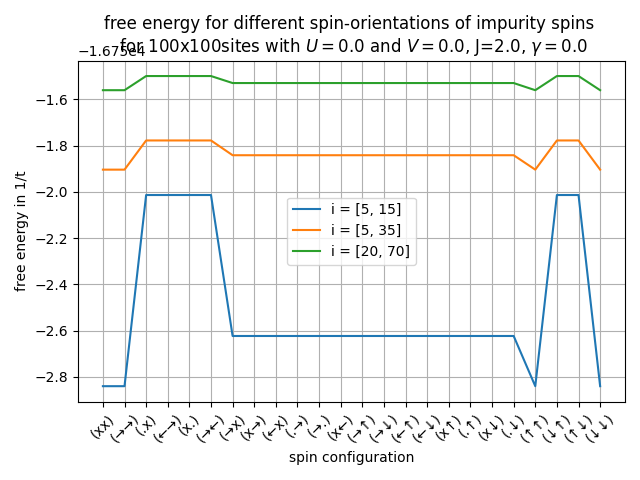
\includegraphics[width=0.48\textwidth]{Images/spinstructure_100_100_0.5_0.0_0.0_0.0_2.0_5_20.png}} \label{fig:spinstruct_nm_J2}
    \subfigure[Spin structure for normal metal with RKKY $J=5$ ]{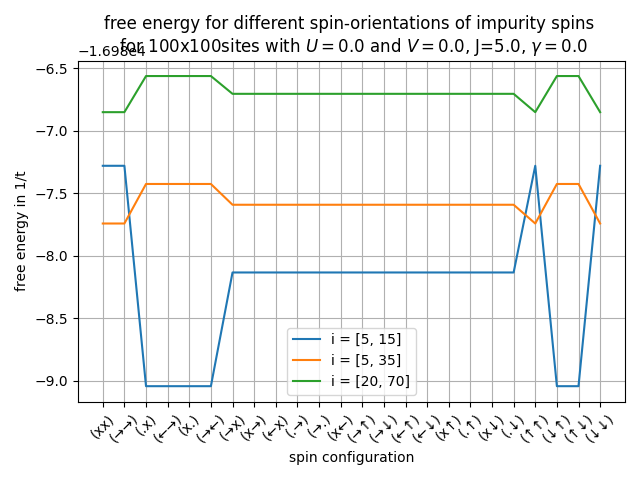
\includegraphics[width=0.48\textwidth]{Images/spinstructure_100_100_0.5_0.0_0.0_0.0_5.0_5_20.png}} \label{fig:spinstruct_nm_J5}
     \caption{The free energy for different impurity spin orientations in a normal metal with RKKY interaction. The Heisenberg form of the RKKY interaction is clearly visible, as well as the dependence on the distance between the impurity spins. (a) has a weaker RKKY interaction than (b), which changes the preferred alignment from parallel to anti-parallel.}
    \label{fig:spinstruct_nm}
\end{figure}

%%%%%%%%%%%%%%%%%%%%%%%%%%%%%%%%%%%%%%%%%%%%%%%%%%%%%%
\section{Normal Metal with SOC and RKKY}\label{sec:RKKY_SOC}

A local spin-orbit coupling (SOC) with coupling strength $\gamma$ is introduced to the normal metal now.
The SOC strength is assumed to be the same in the entire system, which is reasonable since only the bulk properties are of interest here.\textcolor{red}{Do I have something about this in the theory section already? Write down the SOC term for the Hamiltonian anyways}
Employing the Fourier transformation of the fermion operators again, leads to the diagonalized Hamiltonian of the system, which is
\begin{align}
    H_{SOC} = \sum_{k,\sigma, \sigma'} [(\epsilon_k - \mu)\delta_{\sigma \sigma'} + \vb{\gamma}\, \vb{n} \left(\vb{d}_{k} \times \Vec{\sigma}_{\sigma, \sigma'} \right) ] c^{\dag}_{k,\sigma}c_{k,\sigma'}
\end{align}
The Hamiltonian is therefore diagonal in momentum $k$, but not in spin $\sigma$. 
Since the SOC couples spin and momentum, this is to be expected and leads to the definition of the helicity $\lambda$, which expressed exactly this dependency.
As a second step, the fermion operators are therefore transformed from spin-space to helicity-space \cite{samokhin2008gap, mukherjee_soumya_p_superconductivity_2014} by the transformation
\begin{equation}\label{eq:helicitytrafo}
    b_{k,\lambda} = \frac{Z_{k,\lambda}}{\sqrt{2|\gamma_k|}}\left(\sqrt{(|\gamma_k|+\lambda \gamma_{k,z})}c_{k, \uparrow} + \lambda \sqrt{(|\gamma_k|-\lambda \gamma_{k,z})}c_{k,\downarrow}\right)
\end{equation}
where $\lambda= \pm 1$ is the helicity index, $\vb{\gamma}(k) = \gamma_k$ and $Z_{k, \lambda} = 1$ for $\lambda=1$ and $Z_{k, \lambda} = \exp(i\Phi_k)$ for $\lambda=-1$ with
\begin{equation}\label{eq:helicitytrafo_phase}
    \exp(i\Phi_k)=\frac{(\gamma_x + i \gamma_y)}{\sqrt{|\gamma|^2 - \gamma_z^2}}
\end{equation}
being the phase induced by the SOC.
This transformation is unitary and therefore preserves the fermionic anti-commutation relations of the $c$-operators.\newline
Inserting this into the Hamiltonian in Eq.\eqref{eq:hamiltoniankspacekinSOC} leads to the diagonalized expression for the non-centrosymmetric material
\begin{equation}\label{eq:ham_nm+SOC}
    H_{SOC} = \sum_{k,\lambda} \left( (\epsilon_k-\mu) + \lambda |\gamma| \right) b^{\dag}_{k,\lambda}b_{k,\lambda} = \sum_{k, \lambda} \xi_{k, \lambda}b^{\dag}_{k,\lambda}b_{k,\lambda} 
\end{equation}
Therefore the energy spectrum of the spin-orbit coupled electron system in helicity basis is 
\begin{equation} \label{eq:energy_nm+SOC}
    \xi_{k, \lambda} = (\epsilon_k-\mu) + \lambda |\gamma(k)|
\end{equation}
which describes the lift of the spin-degeneracy.
Although each helicity-basis operator $b_{k,\lambda}$ contains both $c_{k,\uparrow}$ and $c_{k,\downarrow}$, they are weighted differently.
That leads to different energies associated with the different spin-orientations. \newline
By employing the SWT again, the spin structure of two impurity spins interacting via RKKY-interaction is found to be
\begin{align}\label{eq:nm_soc_spinStruct}
    \langle H^{RKKY}_{SOC} \rangle = \langle H_{SOC} \rangle + \sum_{i,j,k,k'}  \vb{J}^{SOC}_{i,j,k,k'} \vb{S}_i\vb{S}_j + D^{SOC}_{i,j,k,k'}(S_{i,z}S_{j,x}-S_{i,x}S_{j,z})
\end{align}
where the coefficients $\vb{J}$ and $D$ are defined as
\begin{align}\label{eq:nm_soc_spinCoeffi}
    \vb{J}^{SOC} &= \frac{1}{2}\left(\frac{J}{N}\right) e^{i(k-k')(r_i-r_j)}\left( 
    \begin{array}{c}
         K^{k,k'}_{+,+} +  K^{k,k'}_{-,-} +  K^{k,k'}_{+,-} +  K^{k,k'}_{-,+}\\
          K^{k,k'}_{+,+} +  K^{k,k'}_{-,-} -  K^{k,k'}_{+,-} -  K^{k,k'}_{-,+}\\
         -2 ( K^{k,k'}_{+,-} +  K^{k,k'}_{-,+})
    \end{array}
    \right) \\ \nonumber
    D^{SOC} &=\frac{1}{2}\left(\frac{J}{N}\right) e^{i(k-k')(r_i-r_j)}\left( 
    \begin{array}{c}
         ( K^{k,k'}_{+,-} -  K^{k,k'}_{-,+})\left(\frac{\gamma_{k,x} + i \gamma_{k,y}}{|\gamma_k|} - \frac{\gamma_{k',x} - i \gamma_{k',y}}{|\gamma_k'|}\right)
    \end{array}
    \right)
\end{align}
with $K^{k,k'}_{\lambda, \lambda'} = \frac{f(E_{k,\lambda}) - f(E_{k',\lambda'})}{\xi_{k',\lambda'}-\xi_{k,\lambda}}$ \newline
\textcolor{red}{Adapt notation to the rest of the thesis's notation. Make it fit at this new position. Make it a smooth transition. The following paragraph is an interpretation of the result above}\newline
The RKKY interaction and its spin configuration has been investigated in normal metals with SOC \cite{gong2015dzyaloshinskii, imamura2004twisted, valizadeh_mohammad_m_magnetic_2017}.
In a 2-dimensional electron gas (2DEG), spin orbit coupling results in a twisted RKKY-interaction as shown by Imamura et al. \cite{imamura2004twisted}. 
This is shown by looking at a 2DEG with Rashba-SOC and comparing the results for the spin-structure obtained with the Green's function formalism to the inner product of the untwisted spin space of the first spin and the twisted spin space of the second spin.
Namely, the spin space of the second impurity spin is twisted as
\begin{align} \nonumber
    S_2^x(\theta_{12}) &= \cos{\theta_{12}}S_2^x + \sin{\theta_{12}} S_2^z \\ \nonumber
    S_2^y &= S_2^y \\ \nonumber
    S_2^z &= \cos{\theta_{12}}S_2^z - \sin{\theta_{12}} S_2^x
\end{align}
where the angle $\theta = 2 m\alpha |\vb{R}_1 - \vb{R}_2|$ with the SOC strength $\alpha$. \newline
The inner product with the untwisted spin space of the first impurity spin is consequently
\begin{align}
    \vb{S}_1 \cdot \vb{S}_2(\theta_{12}) = \cos{\theta_{12}} \vb{S}_1 \vb{S}_2 + \sin{\theta_{12}} \left( \vb{S}_1 \times \vb{S}_2 \right)_y + (1- \cos{\theta_{12}}) \vb{S}^y_1 \vb{S}^y_2
 \end{align}
 This corresponds to a Heisenberg-like interaction with strength $\cos{\theta_{12}}$, an Ising-like interaction of strength $(1- \cos{\theta_{12}})$ and the y-component of a Dzyaloshinskii-Moriya interaction term with strength $\sin{\theta_{12}}$. \newline
Therefore, a sign- dependency for the spin-configuration in x- and z-direction is expected, while the y-direction should be symmetric for both spin directions.
The angle dependence also suggests that for no SOC the Heisenberg- like interaction is going to be the only remaining term in the spin-structure. \newline
Gong et al. \cite{gong2015dzyaloshinskii} confirm this result, but use the Schrieffer-Wolff transformation to obtain the effective RKKY interaction in presence of SOC in a 2D optical square lattice. 
The Mott insulator regime is chosen since it allows to focus only on the spin degrees of freedom in this system and an external Zeeman field is added.
With Rashba-type SOC, they find the effective Hamiltonian
\begin{align}\nonumber
    H_{eff} = \sum_{\langle i,j\rangle} \sum_{\alpha = x,y,z} J_{\alpha}S_i^{\alpha}S_j^{\alpha} + \sum_i \vb{B}\cdot \vb{S}_i + \sum_{i,j} \vb{D}_{ij}\cdot\left(\vb{S}_i \times \vb{S}_j \right) + \vb{S}_i \cdot \Gamma \cdot \vb{S}_j
\end{align}
\textcolor{red}{This way of writing the spin structure says nearly nothing about the actual structure, since it allows for all possible combinations of spins}\newline
Since the spin-structure in a superconductor without SOC is of Heisenberg and Ising structure, it is similar to a normal metal without SOC.
Therefore it is to be expected to find a spin-structure of the same type as Imamura et al. and Gong et al. found.\newline
Additionally, the general spin structure for a 2DEG with SOC and RKKY was calculated with the Green's functions approach by Mohammad \cite{valizadeh_mohammad_m_magnetic_2017}.
The notation used in that thesis leads to a spin structure with the three terms identified earlier and reads 
\begin{equation} \label{eq:spinstructure_mohammad}
    H_{eff} = J\,\vb{S}_i \cdot \vb{S}_j + \vb{D}\left( \vb{S}_i \times \vb{S}_j\right) + \vb{S}_i \cdot \overleftrightarrow{\Gamma} \cdot \vb{S}_j
\end{equation}
\textcolor{red}{This notation of the spin structure is not unique, since Mohammad chooses a specific representation for the Green's functions and assigns very specific combinations of them to the coefficients, which is not given naturally from the problem (see Eq.3.7, 3.9, 3.10)}\newline
There is no magnetic field and therefore no Zeeman splitting term present in this approach.
Consequently, this notation is going to be used in this work to denote the different spin terms of a non-centrosymmetric superconductor with RKKY interaction.
\textcolor{red}{Add Mohammad to explanation, add Frigeri for explanation of preferred orientation of spin because of SOC}
Since parts of this spin structure stem solely from SOC, the preferred spin direction can be explained with the direction of the SOC as done by Frigeri et al. \cite{frigeri2004superconductivity}.
In their work, the SOC is defined as $H_{RKKY}^{\text{Frigeri}} = \alpha \sum_{k,s,s'} \vb{g}_{\vb{k}}\sigma_{s,s'} c^{\dag}_{k,s}c_{k,s'}$, where $\sigma$ is the Pauli matrix vector, $s,s'$ are spin indices and $\vb{g}_k = - \vb{g}_{-k}$ is the SOC vector.
This term is embedded into a superconductor that consequently exhibits singlet and triplet pairing.
The coupling depends on the difference of DOS on the two separated Fermi surfaces and therefore is of order $\alpha/\epsilon_F << 1$, where $\epsilon_F$ is the Fermi energy of the higher Fermi surface.
That allows to decouple the singlet and triplet gap equations and to find the transition temperature $T_c$ for singlet and triplet pairing separately.
For the singlet pairing the transition temperature is found to be given by
\begin{equation}\nonumber
    \ln{\left( \frac{T_c}{T_{cs}}\right)} = O\left( \frac{\alpha^2}{\epsilon_F^2} \right)
\end{equation}
which means that the transition temperature essentially is the same with and without SOC. \newline
For the triplet pairing the transition temperature is given by
\begin{align}\label{eq:T_c_triplet}
     \ln{\left( \frac{T_c}{T_{ct}}\right)} = 2\langle \left( |\vb{d}(\vb{k})|^2 - |\vb{g}(\vb{k})\cdot \vb{d}(\vb{k})|^2\right)f(\rho_k) \rangle_k + O\left( \frac{\alpha^2}{\epsilon_F^2} \right)
\end{align}
where $\vb{d}(\vb{k})$ is the normalized triplet gap function and the function $f(\rho)$ is dependent on the SOC, but not relevant for the further argumentation and therefore not specified here.
The highest possible transition temperature is according to Eq. \eqref{eq:T_c_triplet} reached at $T_c = T_{ct}$, which is the case for $\vb{d}(\vb{k}) || \vb{g}_{\vb{k}}$.
This suggests a preferred spin alignment parallel to the SOC and that there might be triplet states, which are unaffected by the lack of inversion symmetry.

\begin{figure}[H]
    \centering
    \subfigure[LDOS for SOC with RKKY $J= 2$ ]{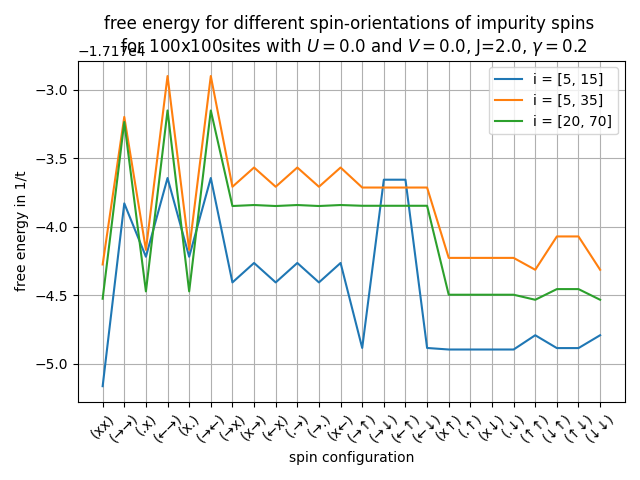
\includegraphics[width=0.48\textwidth]{Images/spinstructure_100_100_0.5_0.0_0.0_0.2_2.0_5_20.png}}
    \subfigure[LDOS for SOC with RKKY $J=5$ ]{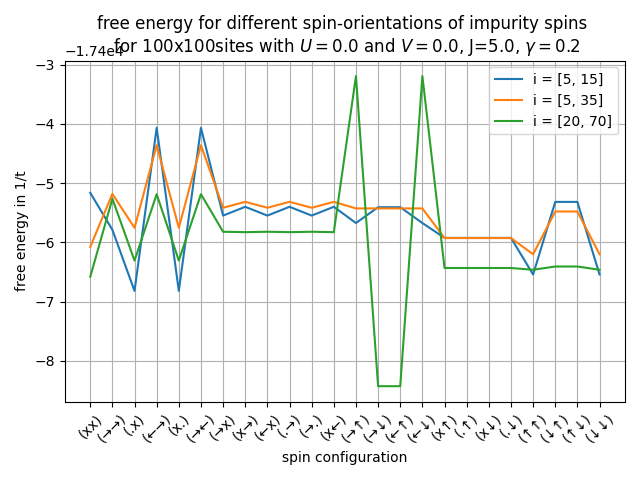
\includegraphics[width=0.48\textwidth]{Images/spinstructure_100_100_0.5_0.0_0.0_0.2_5.0_5_20.png}}
     \caption{The free energy for different impurity spin orientations in a normal metal with SOC and RKKY interaction. The Heisenberg form of the RKKY interaction is clearly visible, as well as the dependence on the distance between the impurity spins.(a) has a weaker RKKY interaction than (b), which changes the preferred alignment from parallel to anti-parallel.}
    \label{fig:spinstruct_nm+SOC}
\end{figure}
%%%%%%%%%%%%%%%%%%%%%%%%%%%%%%%%%%%%%%%%%%%%%%%%%%%%%
\section{Superconductor with RKKY}
\textcolor{red}{Atousa's PhD thesis covers nearly everything}
A superconductor can be described as a normal metal with an additional attractive interaction term between two fermions.
The Hamiltonian consequently takes the from
\begin{align}\nonumber
    H_{SC} = H_{nm} + \sum_i V c^{\dag}_{i,\uparrow}c^{\dag}_{i,\downarrow}c_{i,\downarrow}c_{i,\uparrow}
\end{align}
where $V < 0$ \textcolor{red}{Is it really $<0$?} denotes the strength of the attractive potential, which is a BCS on-site attractive interaction.\newline
As the first step to diagonalize this Hamiltonian, the attractive interaction term is transformed into k-space and a mean-field treatment is performed as introduced in Sec. \ref{sec:BCS}.
$H_{SC}$ reads afterwards
\begin{align} \nonumber
    H_{SC} = \sum_{k,\sigma} (\epsilon_k - \mu)c^{\dag}_{k,\sigma}c_{k,\sigma} - \sum_{k,\sigma}\left[\Delta c^{\dag}_{k,\uparrow}c^{\dag}_{-k,\downarrow} + \Delta^*c_{-k,\downarrow}c_{k,\uparrow}\right] - \frac{|\Delta|^2}{V}
\end{align}
The attractive interaction leads to an s-wave superconductor with $\Delta \in \mathrm{R}$.
\textcolor{red}{How do I know that? Important, so I can later distinguish the p-wave case.}\newline
Secondly, a BdG transformation as described in Sec. \ref{sec:BdG} is applied which defines new fermion operators as
\begin{align}\nonumber
    c_{k,\sigma} &= \eta_k \, \gamma_{k,\sigma} + \sigma\, \nu_k\, \gamma^{\dag}_{-k,-\sigma} \\ \nonumber
    c^{\dag}_{-k,-\sigma} &=  -\sigma\, \nu_k\, \gamma_{k,\sigma} + \eta_k \, \gamma^{\dag}_{-k,-\sigma}
\end{align}
where
\begin{align} \nonumber
    \eta_k =  \frac{(\sqrt{(\epsilon_k-\mu)^2+\Delta^2}+\epsilon_k-\mu)}{\sqrt{(\sqrt{(\epsilon_k-\mu)^2+\Delta^2}+\epsilon_k-\mu)^2+\Delta^2}} \\ \nonumber
    \nu_k = \frac{\Delta}{\sqrt{(\sqrt{(\epsilon_k-\mu)^2+\Delta^2}+\epsilon_k-\mu)^2+\Delta^2}}
\end{align}
and the notation is adapted from Ghanbari \cite{ghanbari_rkky_nodate}. \newline
Ultimately, the diagonalized $H_{SC}$ takes the form
\begin{align}\nonumber
    H_{SC} &= - \frac{|\Delta|^2}{V} + \sum_k (\epsilon_k -\mu) + \sum_{k,\sigma} \sqrt{(\epsilon_k-\mu)^2+\Delta^2} \left( \gamma^{\dag}_{k,\sigma}\gamma_{k,\sigma} - \frac{1}{2}\right) \\ \nonumber
    &=- \frac{|\Delta|^2}{V} + \sum_k (\epsilon_k -\mu) + \sum_{k, \sigma} E^{SC}_{k}\left( \gamma^{\dag}_{k,\sigma}\gamma_{k,\sigma} - \frac{1}{2}\right)
\end{align}
The RKKY interaction is treated perturbatively again and therefore an SWT is applied.
The ansatz $S=\sum_{k,k',\alpha,\beta} (A_{k,k',\alpha,\beta}\gamma^{\dag}_{k,\alpha}\gamma_{k',\beta} + B_{k,k',\alpha,\beta}\gamma^{\dag}_{k,\alpha}\gamma^{\dag}_{-k',-\beta} + C_{k,k',\alpha,\beta}\gamma_{-k,-\alpha}\gamma_{k',\beta} + D_{k,k',\alpha,\beta}\gamma_{-k,-\alpha}\gamma^{\dag}_{-k',\beta})$ is used in the SWT and yields the four coefficients
\begin{align}
    A_{k,k',\alpha,\beta} &= i\sum_i \frac{J}{N}e^{i(k-k')r_i}\left(\vb{S}_i \cdot \Vec{\sigma}_{\alpha,\beta}\right) \frac{\eta^*_k\eta_{k'}}{E_{k'}-E_{k}} \\ \nonumber
    B_{k,k',\alpha,\beta} &= -\beta i\sum_i \frac{J}{N}e^{i(k-k')r_i}\left(\vb{S}_i \cdot \Vec{\sigma}_{\alpha,\beta}\right) \frac{\eta^*_k\nu_{k'}}{E_{-k'}+E_{k}} \\ \nonumber
    C_{k,k',\alpha,\beta} &= \alpha i\sum_i \frac{J}{N}e^{i(k-k')r_i}\left(\vb{S}_i \cdot \Vec{\sigma}_{\alpha,\beta}\right) \frac{\nu^*_k\eta_{k'}}{E_{k'}+E_{-k}} \\ \nonumber
    D_{k,k',\alpha,\beta} &= \alpha \beta i\sum_i \frac{J}{N}e^{i(k-k')r_i}\left(\vb{S}_i \cdot \Vec{\sigma}_{\alpha,\beta}\right) \frac{\nu^*_k\nu_{k'}}{-E_{-k'}+E_{-k}}
\end{align}
Based on this coefficients, the effective interaction $H^{RKKY}_{SC}$ can be calculated. After some algebra, $\langle H^{RKKY}_{SC} \rangle$ is determined and the spin structure can be written in form of Heisenberg interaction:
\begin{align}
    \langle H^{RKKY}_{SC} \rangle = \langle H_{SC} \rangle + \sum_{i,j, k,k'} J^{SC} \vb{S}_i \vb{S}_j
\end{align}
where $J^{SC}$ is defined as 
\begin{align}
    J^{SC} = &\sum_{k,k'} \left( \frac{J}{N} \right)^2 e^{i(k-k')(r_1-r_2)} \\ \nonumber
    &\times \left[ \left(|\eta_k\eta_{k'}|^2 + |\nu_k\nu_{k'}|^2\right) \frac{f(E_k)-f(E_{k'})}{E_{k'}- E_k} -2\eta^*_k\eta_{k'}\nu^*_k \nu_{k'} \frac{f(E_{k'})-f(E_k)}{E_{k'}-E_k}\right]
\end{align}
Numerically, the same spin structure is found as can be seen in Fig. \ref{fig:spin_SConly}
The switch between FM and AFM spin orientation for $J>3.8t$ has the same reasons as in a normal metal.
Additionally, in a superconductor the distance between impurities has consequently no influence, since electrons are conduct perfectly.\newline
Therefore the RKKY interaction strength is kept within $J\in [0, 3.5t]$ to avoid such effects for superconducting systems, too.

\begin{figure}[H]
    \centering
    \subfigure[Spin structure for SC with RKKY $J= 2$ (no SOC) ]{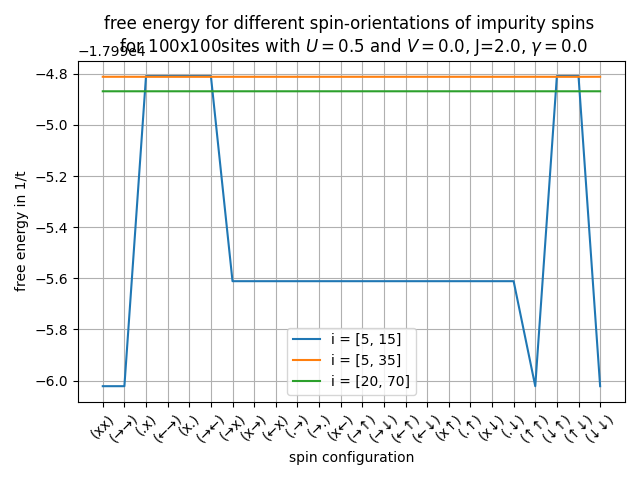
\includegraphics[width=0.48\textwidth]{Images/spinstructure_100_100_0.5_0.5_0.0_0.0_2.0_5_20.png}}
    \subfigure[Spin structure for SC with RKKY $J=5$ (no SOC)]{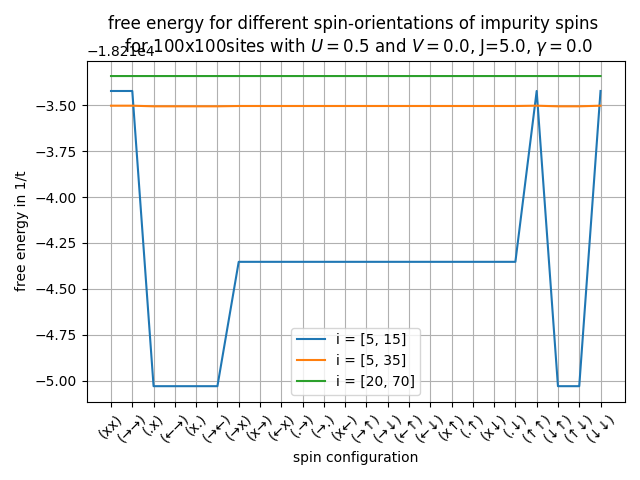
\includegraphics[width=0.48\textwidth]{Images/spinstructure_100_100_0.5_0.5_0.0_0.0_5.0_5_20.png}}
    \caption{The free energy of a superconductor with RKKY interaction for different orientations of the two impurity spins. (a) has a weaker RKKY interaction than (b), which changes the preferred alignment from parallel to anti-parallel.}
    \label{fig:spin_SConly}
\end{figure}


%%%%%%%%%%%%%%%%%%%%%%%%%%%%%%%%%%%%%%%%%%%%%%%%%%%%%
\section{Superconductor with SOC and RKKY}
The interactions within a non-centrosymmetric superconductor can be expressed by the following Hamiltonian:
\begin{equation}\label{eq:hamiltonian0}
    H_{uSC} = H_{SOC} + H_{int}
\end{equation}
The diagonalization of $H_{SOC}$ is already known and written out in Eq. \eqref{eq:ham_nm+SOC}, therefore the attractive interaction between electrons $H_{int}$ has to be added and the final Hamiltonian diagonalized. 
The RKKY interaction is going to be treated as a perturbation to that Hamiltonian. \newline
The attractive interaction term of the non-centrosymmetric superconductor is based on BCS theory and reads in helicity space
\begin{equation}\nonumber
    H_{int} = \sum_{k,k',q} \sum_{\alpha, \alpha', \beta, \beta'} -\frac{1}{2} V_{\alpha, \alpha', \beta, \beta'}(k,k',q) b^{\dag}_{k,\alpha} b^{\dag}_{-k+q,\beta} b_{-k'+q,\beta'}b_{k', \alpha'}
\end{equation}
where $\alpha,\beta$ are helicity-band-indices and $V_{\alpha, \alpha', \beta, \beta'}(k,k',q)$ denotes the interaction strength. 
The SOC is assumed to be large compared to the size of the gaps, which suppresses interband hopping.
\textcolor{red}{Maybe: Reference numerical study on what this actually means}\newline
Therefore, the helicity indices are set to $\alpha = \beta = \lambda$ and $\alpha' = \beta' = \lambda'$.\newline %\cite{taraldsen_oyvind_muldal_quantum_2021}
Since the phase space changes with the value of $q$ and is maximal for $q=0$, all other contributions are negligibly small for large enough SOC \cite{samokhin2004cept, samokhin2008gap}. \newline
This leads to the following expression of the interaction term
\begin{equation}\label{eq:hamiltoniankspaceint}
    H_{int} = \sum_{k,k'} \sum_{\lambda, \lambda'} -\frac{1}{2} V_{\lambda, \lambda'}(k,k') b^{\dag}_{k,\lambda} b^{\dag}_{-k,\lambda} b_{-k',\lambda'}b_{k', \lambda'}
\end{equation}
which allows for intraband pairing as well as pair-hopping.
\newline
%%%%%%%%%%%%%%%%%%%%%%%%%%%%%%%%%%%%%%%%%%%%%%%%%%%%%%%
Next, a mean-field approximation is done by introducing the average $a_{k,\lambda} = \averg{b_{-k,\lambda}}{b_{k,\lambda}}$. 
The deviation from this average is assumed to be small in the system, such that the approximation $b_{-k,\lambda}b_{k,\lambda}=a_{k,\lambda} + \delta_{k, \lambda}$ holds, when disregarding terms of order $\delta^2$.\newline
This allows to rewrite the Hamiltonian \eqref{eq:hamiltoniankspaceint} as
\begin{equation}
    H_{int} = \sum_{k,k',\lambda, \lambda'} -\frac{1}{2}V_{\lambda, \lambda'}(k,k') \left[ 
    a^{\dag}_{k,\lambda}b_{-k',\lambda'}b_{k', \lambda'} + 
    a_{\lambda'}(k')b^{\dag}_{k,\lambda} b^{\dag}_{-k,\lambda} - a^{\dag}_{\lambda}(k)a_{k',\lambda'} \right]
\end{equation}
By defining the order parameter
\begin{equation}
    \Delta_{k, \lambda} = \sum_{\lambda', k'} V_{\lambda, \lambda'}(k,k') a_{k',\lambda'}
\end{equation}
which is called gap in the BCS theory, the Hamiltonian \eqref{eq:hamiltoniankspaceint} can be further rewritten into the form
\begin{equation} \label{eq:hamiltoniankspaceint_MF}
    H_{int} = -\sum_{k,\lambda} \frac{1}{2} \left[\Delta_{k, \lambda}b^{\dag}_{k,\lambda} b^{\dag}_{-k,\lambda} +\Delta^{\dag}_{k, \lambda} b_{-k,\lambda} b_{k,\lambda}\right] + \Delta_{k, \lambda}a^{\dag}_{k,\lambda}
\end{equation}
where the last term is constant and is going to be disregarded for now.
%%%%%%%%%%%%%%%%%%%%%%%%%%%%%%%%%%%%%%%%%%%%%%%%%%%%%%%
\subsection{Singlet and Triplet Pairing Interaction}
% used resources \cite{taraldsen_oyvind_muldal_quantum_2021} and \cite{Ikegaya_2021_tunableMajorana} \newline
The attractive interaction between electrons in a non-centrosymmetric superconductor does not only lead to spin-singlet pairs but also to spin-triplet pairs [QUELLE]. 
The Hamiltonian for attractive electron interaction in the helicity basis is introduced in Eq. \ref{eq:hamiltoniankspaceint} and treated with a mean field approach it reads
\begin{equation}
    H_{int} = -\frac{1}{2} \sum_{k,\lambda}\left( \Delta_{k,\lambda} b^{\dag}_{k,\lambda}b^{\dag}_{-k,\lambda} + h.c.\right)
\end{equation}
where the constant term is neglected (compare Eq. \ref{eq:hamiltoniankspaceint_MF}).\newline
The Hamiltonian including tight binding model and spin-orbit-coupling is diagonalized by fermionic operators in helicity space and its eigen-energies are symmetric in k.
That allows to write the operation of the time-reversal operator $K = i \sigma_y K_0$, where $K_0$ is the complex conjugation, acting on a state $|k,\lambda\rangle$ as $K|k,\lambda\rangle = t_{k,\lambda} |-k,\lambda\rangle$ \cite{samokhin2008gap}.
Here, the nontrivial phase factor $t_{k,\lambda}$ is defined and for the eigenbasis in helicity space it reads
\begin{equation}\label{eq:phasefactor_t}
    t_{k,\lambda} = \lambda \frac{\gamma_{k,x} - i \gamma_{k,y} }{|\gamma_k|}
\end{equation}
and therefore depends on the lattice symmetry as well as the chosen type of SOC.
Note that this is exactly the phase factor introduced for the basis transformation between the fermion operators in spin-space and helicity space in Eq. \ref{eq:helicitytrafo_phase} \newline
The phase factor allows to write the interaction potential and the gap as 
\begin{align}\label{eq:int_potential_delta_phase}
    V_{k,k',\lambda, \lambda'} &= t_{k,\lambda}t^*_{k',\lambda'} \Tilde{V}_{k,k',\lambda, \lambda'} \\
    \Delta_{k,\lambda} &= t_{k,\lambda}\Tilde{\Delta}_{k,\lambda}
\end{align}
In addition, it is possible to split the gap in the spin-space into positive and negative helicity parts 
\begin{align}\label{eq:gap_tri_spinbasis}
    \Delta_{k, \sigma, \sigma'} &= \left[ \left(\Delta_{s,k} + \vb{d}_k\vb{\sigma}\right)i\sigma_y\right]_{\sigma, \sigma'} \\ \nonumber
    \Delta_{s,k} &= \frac{\Tilde{\Delta}_{k,+} + \Tilde{\Delta}_{k,-} }{2} \\ \nonumber
    \vb{d}_k &= \frac{\Tilde{\Delta}_{k,+} - \Tilde{\Delta}_{k,-} }{2} \vb{\gamma}_k = \Delta_{t,k} \frac{\vb{\gamma}_k}{|\vb{\gamma}_k|}
\end{align}
This is a 2x2 matrix expressed in helicity basis variables for the different possible spin-configurations.
Furthermore, the definition of $\vb{d}_k$ implies that only the orientation parallel to the SOC is allowed. 
\newline
In the case of Rashba-SOC, it is possible to specify the expression for $\vb{d}_k$ in terms of the SOC vector $\vb{\gamma}_k$ and the triplet-pairing strength $\Delta_t$ \cite{Ikegaya_2021_tunableMajorana}, so that the total gap reads in spin-space
\begin{align}\label{eq:gap_singlet+triplet}
    \Delta_k = \left(
    \begin{array}{cc}
        -i\frac{\Delta_{t,k}}{|\vb{\gamma}_k|}(k_x + i k_y) &  \Delta_{s,k} \\
        -\Delta_{s,k} & i\frac{\Delta_{t,k}}{|\vb{\gamma}_k|}(k_y - ik_x) 
    \end{array}
    \right)
\end{align}
For a square lattice, the interaction potential can be expressed as a 2x2 matrix of the structure \cite{samokhin2008gap}
\begin{align} \label{eq:couling_tri}
    \Tilde{V}_{k,k', \lambda, \lambda'} &= \frac{1}{2} V_g \left( \sigma_0 + \sigma_x \right) + \frac{1}{2} \lambda \lambda' V_{u,k,k'} \left( \sigma_0 - \sigma_x\right) \\ \nonumber
    &= \left[
    \begin{array}{cc}
       \Tilde{V}^d_{k,k', \lambda, \lambda'}  & \Tilde{V}^o_{k,k', \lambda, \lambda'}  \\
         \Tilde{V}^o_{k,k', \lambda, \lambda'} & \Tilde{V}^d_{k,k', \lambda, \lambda'}
    \end{array}
    \right]
\end{align}
where $V_{g[u]}$ represents the even [odd] parts of the interaction in spin-basis. 
The case of only singlet-pairing corresponds to $V_u = 0$ and $V_g \neq 0$. 
%The diagonal $V^d$ and off-diagonal $V^o$ elements are constants and generally different. \newline

Furthermore holds for a square lattice that SOC generally is $\vb{\gamma}(\vb{k}) = \gamma_0 \vb{k}$ and an attractive interaction is most likely mediated by phonons, which leads to a $k$-independent even part $V_g$.
The resulting gap function is isotropic, because phonons lead to local interactions in most cases.
The magnitudes of the gaps corresponding to the different helicity bands can generally be different and their difference depends on the strength of the spin-orbit coupling \cite{samokhin2008gap}.
Their ratio determines the ratio $|\vb{d}_k|/|\Delta_{s,k}|$ and suggests that for weak SOC singlet-pairing dominates while triplet-pairing dominates for strong SOC. \newline

\textcolor{red}{What do I expect to be the influence of the triplet pairing on the RKKY?} \newline
Since the triplet-pairing mode allows for non-zero spin of Cooper pairs, these Cooper pairs can potentially influence the RKKY interaction.
Single electrons and Cooper pairs have different movement behaviors, which can lead to differences in the RKKY interaction caused by the triplet-pairs.
\textcolor{red}{They are an effect of SOC, which in itself has already an impact or not???}

Taking the triplet-pairing into account alters the shape of the gap expected to be seen in the density of states.
For singlet pairing, there is one region close to $E=0$ where the density of states becomes zero.
It is clearly visible for a large enough attractive potential $U$ and the typical shape can be seen in Fig. \ref{fig:gap_shape_general} when looking at the continuous line.
The dotted line depicts the gap when influenced by triplet-pairing. 
There the shape changes to two overlapping gaps, which can be seen by the step-like behavior of the density of states next to the singlet gap.

\begin{figure}
    \centering
    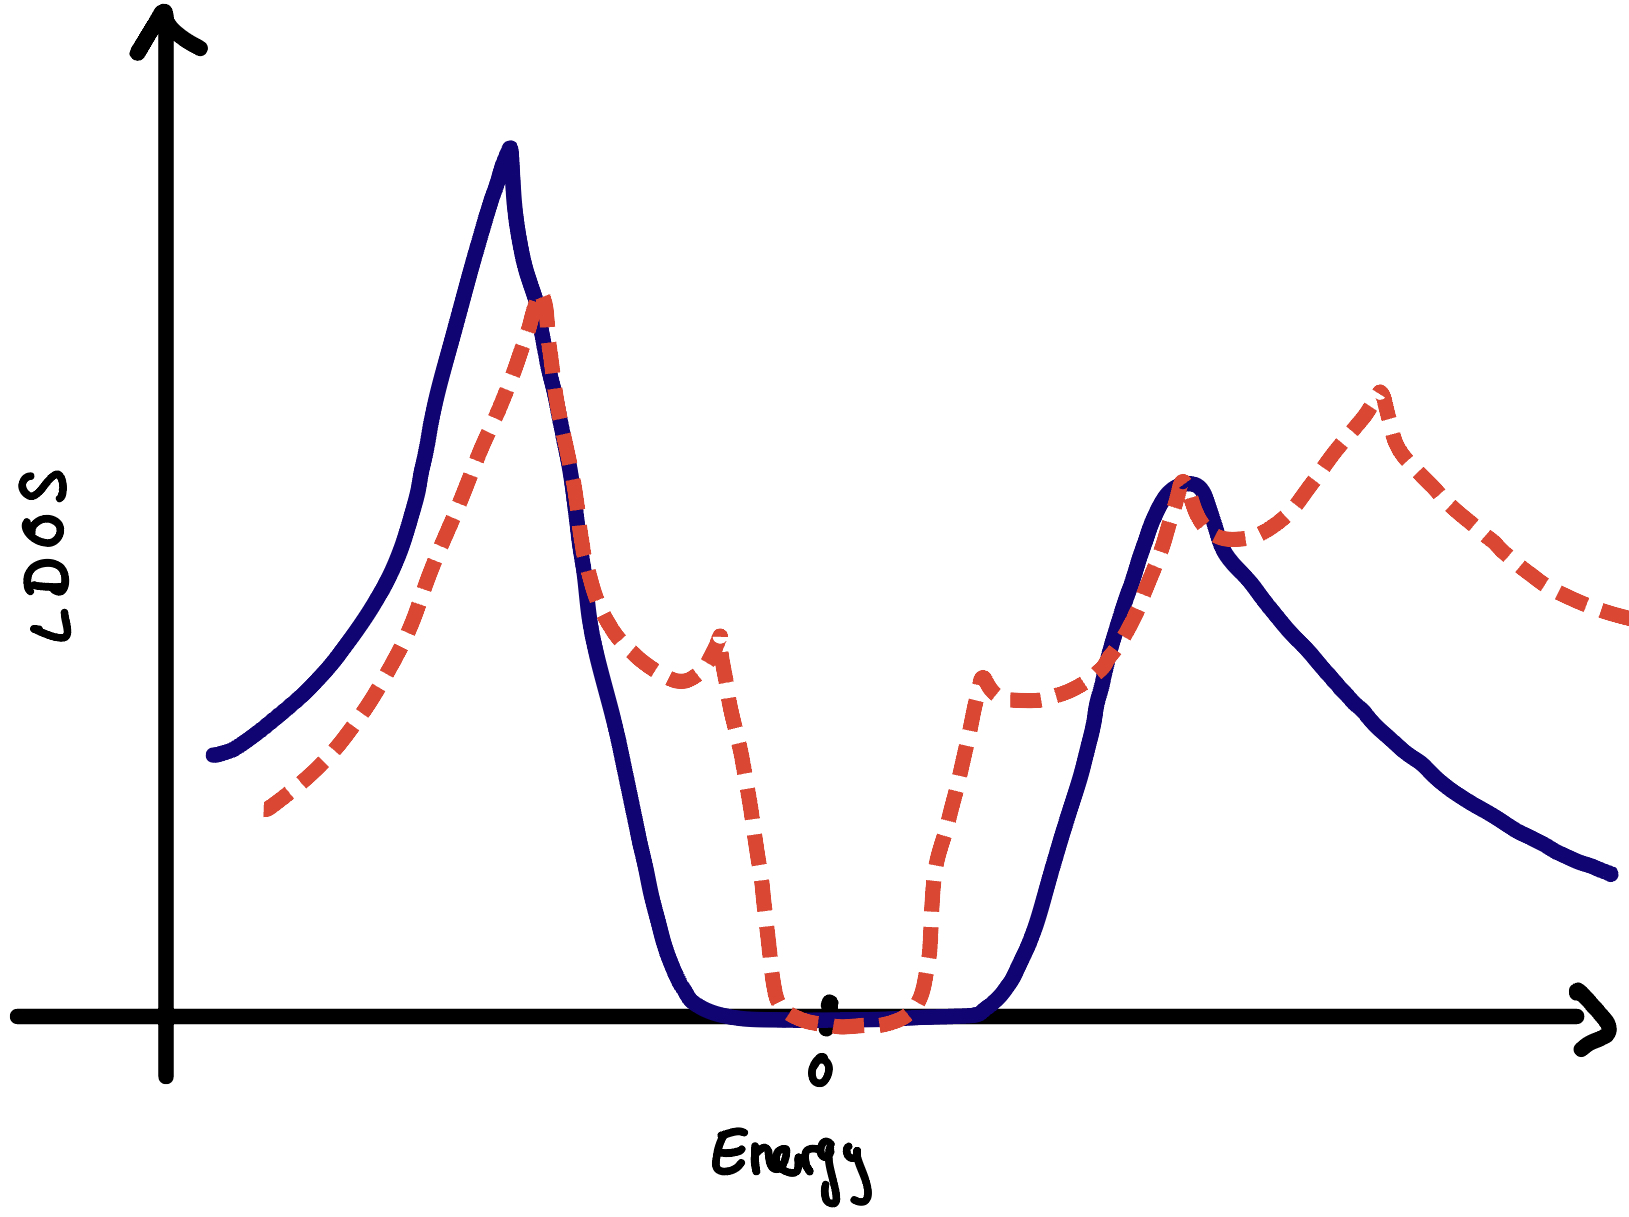
\includegraphics[width=0.8\textwidth]{Images/FDB0FF39-C759-4473-8DBA-F65EB632BAAA.jpeg}
    \caption{General behavior of singlet-pairing (blue, continuous) and triplet-pairing (red, dashed) superconducting gaps. \textcolor{red}{This should be replaced by one of my python graphs and the characteristics explained with the help of that. I also need another reference to make this point, best one with nice graphs.}}
    \label{fig:gap_shape_general}
\end{figure}

%%%%%%%%%%%%%%%%%%%%%%%%%%%%%%%%%%%%%%%%%%
\subsection{Diagonalization}
Combining all individual terms of the Hamiltonian, the system can be described by
\begin{align}
        H_0 &= H_{kin} + H_{pot}+ H_{SOC} + H_{int} \nonumber\\
        &= \label{eq:hamiltonian0matrix} \sum_{k, \lambda} \frac{1}{2} \phi_{k}^{\dag} 
        \left[ {\begin{array}{cc}
            \xi_{k,\lambda} & -\Delta_{k, \lambda} \\
          -\Delta^{\dag}_{k, \lambda} & -\xi_{-k,\lambda} \\
        \end{array} } 
        \right] 
    \phi_{k} + \sum_k \xi_k % + \Delta_{\alpha, \beta}(k)a^{\dag}_{\beta,\alpha}(k)
\end{align}
with the basis vectors $\phi^{\dag}_k = ( b^{\dag}_{k,\lambda}, b^{\dag}_{-k,\lambda})$ and $\phi_k$ its complex conjugate. \newline
This matrix can easily be diagonalized and has eigenvalues 
\begin{align}
    E^{\pm}_{k,\lambda} = \pm \sqrt{\xi^2_{k,\lambda} + |\Delta_{k, \lambda}|^2} %\\
    %F^{\pm}_{\alpha,\beta} (k,q) = \pm \sqrt{\frac{1}{4}\xi_{k,\beta} +\Delta^{\dag}_{k, \lambda}\Delta__{k, \lambda}}
\end{align}
which have been simplified by using that time reversal symmetry is preserved $\epsilon_k = \epsilon_{-k}$.\newline 
The components of the eigenvectors are 
\begin{align}
    \eta_{k,\lambda} = \frac{E^+_{k,\lambda} + \xi_{k,\lambda}}{\sqrt{(E_{k,\lambda} + \xi_{k,\lambda})^2+|\Delta_{k, \lambda}|^2}} \\
    \nu_{k,\lambda} = \frac{\Delta_{k, \lambda}}{\sqrt{(E_{k,\lambda} + \xi_{k,\lambda})^2+|\Delta_{k, \lambda}|^2}}
\end{align}
and the eigenvectors read $\text{v}^{\dag}_1 = (\eta_{k,\lambda}, \nu_{k,\lambda})$ and $\text{v}^{\dag}_2 = (\nu^{\dag}_{k,\lambda}, \eta_{k,\lambda})$ \cite{ghanbari_rkky_nodate}. \newline
The diagonalized Hamiltonian can therefore expressed in the form of a Fermi-gas
\begin{equation}\label{eq:hamiltonian0diag}
    H_0 = \sum_{k, \lambda} \left[ E^{+}_{k, \lambda} (d^{\dag}_{k,\lambda}d_{k,\lambda}-d^{\dag}_{-k,\lambda}d_{-k,\lambda} )\right]  +  \frac{|\Delta|^2}{V} +\sum_k \xi_k - \sum_k E_k %\Delta_{k, \lambda}a^{\dag}_{k,\lambda}
\end{equation}
where $d^{[\dag]}$ is the annihilation [creation] operator for the quasi-particles that diagonalize the total Hamiltonian.
They are defined via the transformation from the helicity basis with matrix $P_{k,\lambda}$, which contains the eigenvectors as columns. 
\begin{align} \label{eq:d_basis_def}
 \left( {\begin{array}{c}
            d_{k, \lambda}\\
          d^{\dag}_{-k, \lambda} \\
        \end{array} } 
        \right)
    = \left[ {\begin{array}{c}
            \eta_{k, \lambda} b_{k, \lambda} + \nu^{\dag}_{k, \lambda}b^{\dag}_{-k, \lambda} \\
          \nu_{k, \lambda}b_{k, \lambda} + \eta_{k,\lambda}b^{\dag}_{-k, \lambda} \\
        \end{array} } 
        \right] 
\end{align}
The anti-commutation-relations of the $d$-operators are fermionic again, since $P_{k,\lambda}$ is unitary.

%%%%%%%%%%%%%%%%%%%%%%%%%%%%%%%%%%%%%%%%%%%%%%%%%%%%%%%%%%%%%%%%%%%%%%%%

\subsection{Free Energy and Gap Equation} \label{sec:free_energy}
The Hamiltonian in Eq. \eqref{eq:hamiltonian0diag} has the form of a Fermi-gas, so the partition function can be calculated based on 
\begin{equation}
    Z = \prod_{k, \lambda} \left( 1 + e^{-\beta E_{k, \lambda}}\right)\left( 1 + e^{\beta E_{k, \lambda}}\right)e^{-\beta \Delta_{k, \lambda}a^{\dag}_{k, \lambda}+\sum_k \xi_k - \sum_k E_k}
\end{equation}
where $\beta = 1/k_B T$, when it is not an index, and $E_{k, \lambda}= E^+_{k, \lambda}$ \cite{sudbo_asle_superconductivity_2004}.\newline
From that the free energy can be calculated as $F = - \frac{1}{\beta}\ln(Z)$ with $ln()$ being the natural logarithm.\newline
The gap function is the functional derivative of the free energy with respect to the order parameter i.e. gap $\Delta_{k, \lambda}$:
\begin{align}
    & \frac{\partial F}{\partial \Delta_{k, \lambda}} \\ \nonumber
    &= -\frac{1}{\beta} \frac{\partial}{\partial \Delta_{k, \lambda}} \sum_{k, \lambda} \left[ \ln\left( 1 + e^{-\beta E_{k, \lambda}}\right) + \ln \left( 1 + e^{\beta E_{k, \lambda}}\right)+ \ln \left( e^{-\beta \Delta_{k, \lambda} a^{\dag}_{k, \lambda}+\sum_k \xi_k - \sum_k E_k}\right)  \right] \\
    &= \frac{\partial E_{k, \lambda}}{\partial \Delta_{k, \lambda}}\left( \frac{e^{-\beta E_{k, \lambda}}}{1 + e^{-\beta E_{k, \lambda}}} - \frac{e^{\beta E_{k, \lambda}}}{1 + e^{\beta E_{k, \lambda}}}\right) + \frac{\partial}{\partial \Delta_{k, \lambda} }\left( \Delta_{k, \lambda} a^{\dag}_{k, \lambda} +\sum_k \xi_k - \sum_k E_k \right) \nonumber \\
    &= \frac{\partial E_{k, \lambda}}{\partial \Delta_{k, \lambda}}\tanh{\left( \frac{\beta E_{k, \lambda}}{2}\right)} + \frac{\partial}{\partial \Delta_{k, \lambda} } \left( \Delta_{k, \lambda} a^{\dag}_{k, \lambda} +\sum_k \xi_k - \sum_k E_k \right) \nonumber \\
    &= \frac{\Delta^{\dag}_{k, \lambda}}{2 E_{k, \lambda}}\tanh{\left( \frac{\beta E_{k, \lambda}}{2}\right)} - a^{\dag}_{k, \lambda} \label{eq:gapequationDerivative}
\end{align}
Changing the derivative and identifying the $\tanh$ lead to the final expression in Eq. \eqref{eq:gapequationDerivative}.\newline
Setting this to zero allows to find the extrema of the free energy. 
Since the free energy is always bound from below, there is at least one minimum to find. 
In order to make sure that the found extremum is that minimum, one has to reinsert the following expression of the gap equation into the free energy:
\begin{align}
    0 &= -\sum_{k, \lambda} V_{k,k', \lambda, \lambda'}\left[ \frac{\Delta^{\dag}_{k, \lambda}}{4 E_{k, \lambda}}\tanh{\left( \frac{\beta E_{k, \lambda}}{2}\right)} - a^{\dag}_{k, \lambda}\right] \nonumber \\ \label{eq:selfconsistencyGap}
    \Leftrightarrow \Delta^{\dag}_{k, \lambda} &= - \sum_{k, \lambda} V_{k',k', \lambda, \lambda'}\frac{\Delta^{\dag}_{k, \lambda}}{4 E_{k, \lambda}}\tanh{\left( \frac{\beta E_{k, \lambda}}{2}\right)}
\end{align}
The complex conjugate of the gap equation can be acquired the same way as this one, but the derivative of the free energy is taken with respect to $\Delta^{\dag}_{k, \lambda}$.
%%%%%%%%%%%%%%%%%%%%%%%%%%%%%%%%%%%%%%%%%%%%%%%%%%%%%%%%%%%%%
\subsubsection{Andreev Reflection} \label{sec:andreev}

\textcolor{red}{Add explanation of Andreev states and explanation for when they are present by Eschrig. \newline Explanation of Anreev is missing completely!}\newline
\textcolor{blue}{It as something to do with electron (hole) approaching a material, where there is a gap while there is no gap in energy in the current system, which leads to the electron (hole) to be reflected as a hole (electron), while a Cooper pair is formed in the material that has the energy gap. \cite{ghanbari_rkky_nodate}} \newline
In a superconducting system that allows for triplet pairing, the surface states are strongly influenced by the relative magnitude of the singlet and triplet gap order parameter $\Delta_s$ and $\Delta_t$, respectively.\newline
To see that, the surface or boundary conditions in wave function formalism are defined by setting the wave function to zero at the boundary.
Based on that the bound state condition can be expressed in dependence of singlet and triplet gap as well as the energy of the system and a proportionality constant $\xi \leq 1$ \cite{eschrig2010theoretical}.
This bound state condition reads
\begin{align}\nonumber
    \sqrt{(\Delta_1^2-E^2)(\Delta_2^2-E^2)} &= \frac{1-\xi}{1+\xi}(E^2+\gamma\Delta_1\Delta_2) \\ \nonumber
    \xi &= 1 \quad \text{for} \quad \Theta_c < |\Theta_2| \leq \pi/2 \\ \nonumber
    \xi &= \frac{\sin^2(\frac{1}{2}[\Theta_1+\Theta_2])}{\cos^2(\frac{1}{2}[\Theta_1-\Theta_2])} \quad \text{for} \quad |\Theta_2| \leq \Theta_c
\end{align}
with $\xi \leq 1$, $\cos\Theta_1 = k_{1x}/k_1$ and $\cos\Theta_2 = k_{2x}/k_2$. And the critical angle $\Theta_C= \arcsin{(k_1/k_2)}$. \newline
Therefore, the proportionality constant depends on the relative magnitude of singlet and triplet gap. The bound state condition reveals that only for $|\Theta_2| \leq \Theta_c$ and $\gamma =1$ zero-energy states are possible. Consequently, they do only appear when the triplet gap is larger than the singlet gap $\Delta_s < \Delta_t$.
\textcolor{red}{This has to be more detailed, since it is going to be a check for my program.}